% sections/02_selection.tex: generated by newdeck/html2beamer.py from the HTML deck, then edited by hand

% ---------------------------------------------------------------- slide 12: Outline
\begin{btframe}{}{Outline}
\begin{outlinelist}
\outlineitem{1}{Introduction}{the background types, the geometry, the input muons and neutrinos}{0.35}
\outlineitem{2}{Simulation}{transport, inelastic scattering, technologies, hits and digitisation, signal generation}{0.35}
\outlineitem{3}{Selection}{track cuts, pair cuts and time coincidence}{1.00}
\outlineitem{4}{Backgrounds before tagging}{μ and ν inelastic scattering, MS7 K\textsubscript{L}, combinatorial pairs}{0.35}
\outlineitem{5}{Background tagging}{rules, V0 rule, SBT model, R1, R2, summary}{0.35}
\outlineitem{6}{Optimisation and conclusion}{genetic-algorithm search, the optimised designs Z2 and Z3}{0.35}
\end{outlinelist}
\end{btframe}

% ---------------------------------------------------------------- slide 13: Track cuts: what a good track is
\begin{btframe}{3 · Selection · tracks}{Track cuts: what a good track is}
\noindent \begin{minipage}[c]{0.4\linewidth}
{\centering 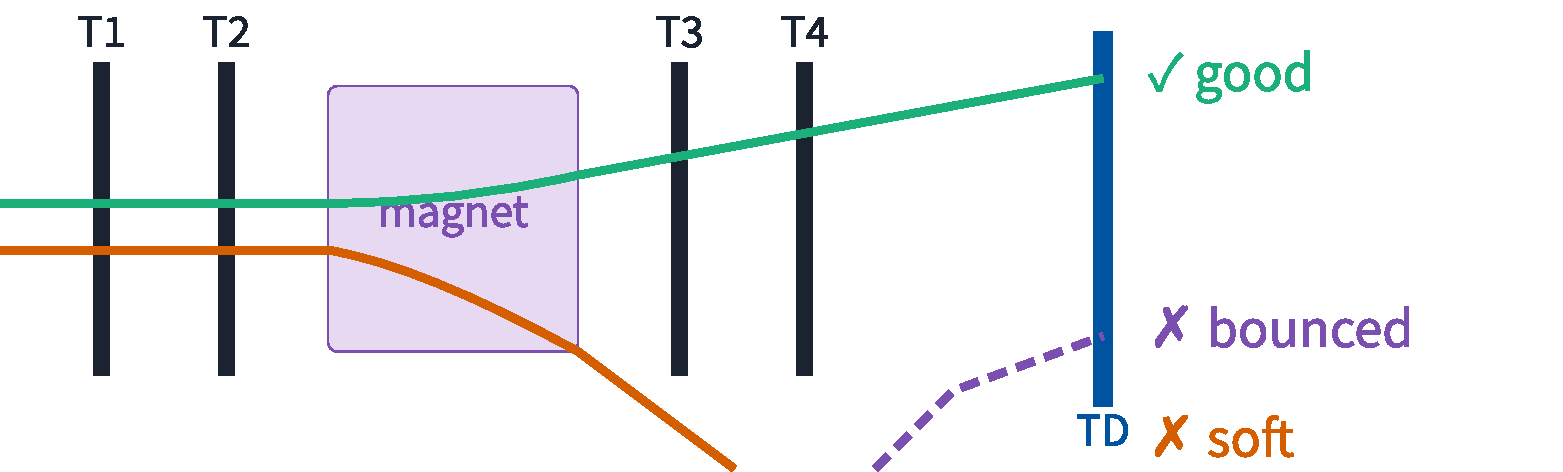
\includegraphics[width=1.00\linewidth,keepaspectratio]{figs/s12_sk1.pdf}\par}
\end{minipage}%
\hfill%
\begin{minipage}[c]{0.6\linewidth}
{\centering 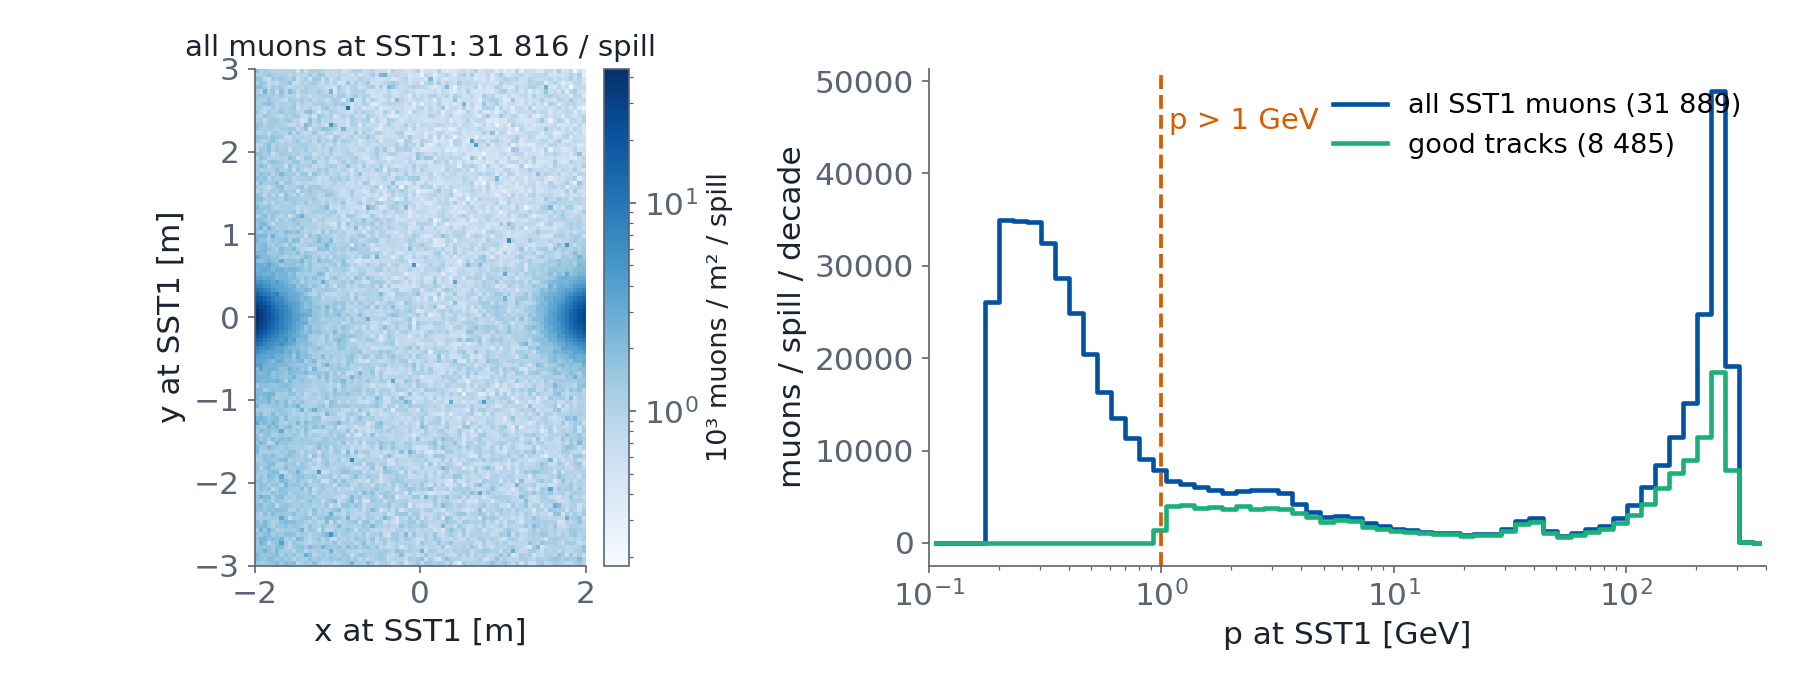
\includegraphics[width=1.00\linewidth]{figs/s12_img2.png}\par}
\end{minipage}\par
\vspace{2.46pt}
{\fontsize{6.02pt}{7.83pt}\selectfont\setlength{\tabcolsep}{4.21pt}\renewcommand{\arraystretch}{1.42}
\begin{tabularx}{\linewidth}{ll>{\raggedright\arraybackslash}Xr}
\textcolor{muted}{\#} & \textcolor{muted}{cut} & \textcolor{muted}{value} & \textcolor{muted}{muons / spill} \\\headrule
1 & SST1 acceptance & |x| < 2, |y| < 3 m at z = 82.08 m & 31.9 kHz \\\rowrule
2 & timing-detector acceptance & through the field map to z = 94.01 m, |x| < 2.75, |y| < 3.25 m &  \\\rowrule
3 & momentum & p > 1 GeV & 8.5 kHz good tracks (8.17 straight + 0.38 bounced) \\\rowrule
– & track quality (ACTS) & converged, n\textsubscript{dof} > 25, χ\textsuperscript{2}/n\textsubscript{dof} < 5 & not yet measured (option, not applied) \\\rowrule
\end{tabularx}\par}
\end{btframe}

% ---------------------------------------------------------------- slide 14: Pair cuts: opposite charge, DOCA, vertex, IP
\begin{btframe}{3 · Selection · pair cuts}{Pair cuts: opposite charge, DOCA, vertex, IP}
\noindent \begin{minipage}[c]{0.75\linewidth}
{\centering 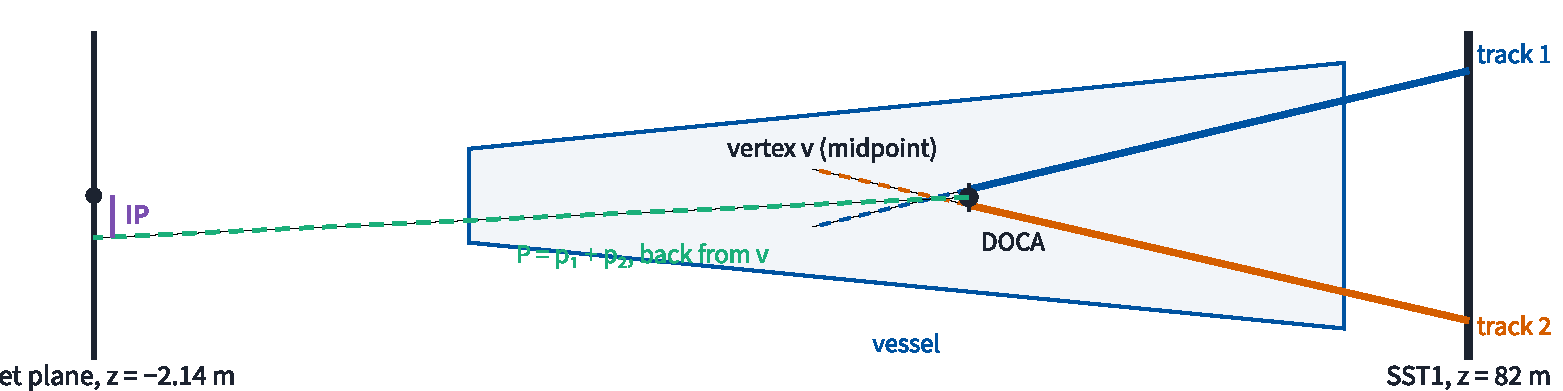
\includegraphics[width=1.00\linewidth,height=54.62pt,keepaspectratio]{figs/s13_sk1.pdf}\par}
\end{minipage}%
\hfill%
\begin{minipage}[c]{0.25\linewidth}
\begin{mathbox}[cern]{4.55pt}
\[\mathrm{DOCA} = \frac{\left|\,\Delta\vec r\cdot(\vec p_1\times\vec p_2)\,\right|}{\left|\vec p_1\times\vec p_2\right|}\]
\end{mathbox}
\vspace{1.64pt}
\begin{mathbox}[cern]{4.32pt}
\[\begin{aligned} \vec P &= \vec p_1 + \vec p_2 \\ \mathrm{IP} &= \left|\,\vec v_{xy} + \frac{\vec P_{xy}}{P_z}\,(-2.14\,\mathrm{m} - v_z)\right| \end{aligned}\]
\end{mathbox}
\end{minipage}\par
\vspace{2.46pt}
{\centering 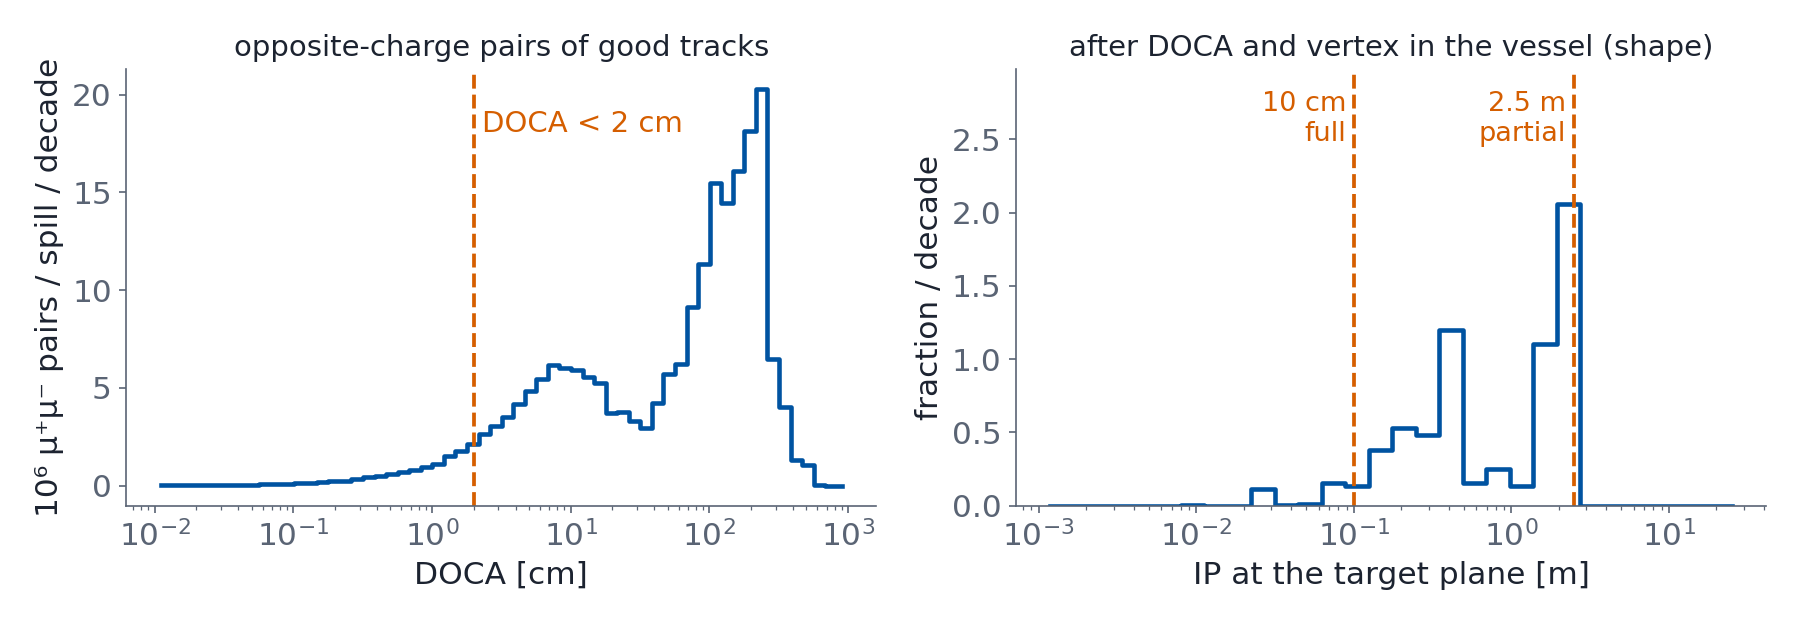
\includegraphics[width=0.66\linewidth]{figs/s13_img2.png}\par}
\vspace{2.46pt}
{\centering \fontsize{7.01pt}{8.76pt}\selectfont \textbf{Time}: two unrelated muons must agree within ±200 ps (TD, σ\textsubscript{t} = 100 ps) over a 1 s spill → factor 2 × 200 ps / 1 s = \textbf{4×10\textsuperscript{-10}}.\par}
\end{btframe}
